
\documentclass{standalone}
\usepackage{tikz}
\begin{document}
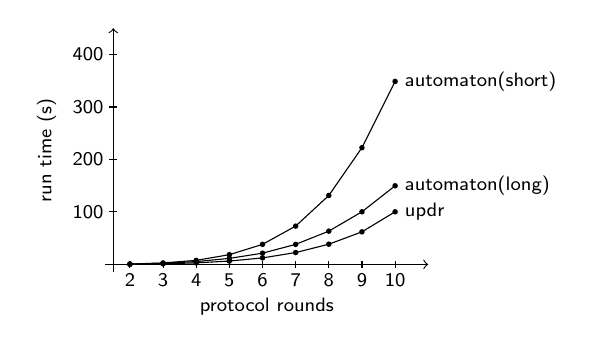
\begin{tikzpicture}[
    lbl/.style={font=\sffamily\scriptsize}
]
    
\draw[->] (-0.1, 0) -- node[lbl,below=3mm] {protocol rounds} (4, 0);
\draw (0.211, -0.05) -- node[lbl,below] {2} (0.211, 0.05);
\draw (0.632, -0.05) -- node[lbl,below] {3} (0.632, 0.05);
\draw (1.053, -0.05) -- node[lbl,below] {4} (1.053, 0.05);
\draw (1.474, -0.05) -- node[lbl,below] {5} (1.474, 0.05);
\draw (1.895, -0.05) -- node[lbl,below] {6} (1.895, 0.05);
\draw (2.316, -0.05) -- node[lbl,below] {7} (2.316, 0.05);
\draw (2.737, -0.05) -- node[lbl,below] {8} (2.737, 0.05);
\draw (3.158, -0.05) -- node[lbl,below] {9} (3.158, 0.05);
\draw (3.579, -0.05) -- node[lbl,below] {10} (3.579, 0.05);
\draw[->] (0, -0.1) -- node[lbl,above=6mm,sloped] {run time (s)} (0, 3);
\draw (-0.05, 0.667) -- node[lbl,left] {100} (0.05, 0.667);
\draw (-0.05, 1.333) -- node[lbl,left] {200} (0.05, 1.333);
\draw (-0.05, 2.0) -- node[lbl,left] {300} (0.05, 2.0);
\draw (-0.05, 2.667) -- node[lbl,left] {400} (0.05, 2.667);
\fill[] (0.211, 0.005) circle [radius=1pt];
\fill[] (0.632, 0.015) circle [radius=1pt];
\draw[] (0.211, 0.005) -- (0.632, 0.015);
\fill[] (1.053, 0.036) circle [radius=1pt];
\draw[] (0.632, 0.015) -- (1.053, 0.036);
\fill[] (1.474, 0.077) circle [radius=1pt];
\draw[] (1.053, 0.036) -- (1.474, 0.077);
\fill[] (1.895, 0.143) circle [radius=1pt];
\draw[] (1.474, 0.077) -- (1.895, 0.143);
\fill[] (2.316, 0.255) circle [radius=1pt];
\draw[] (1.895, 0.143) -- (2.316, 0.255);
\fill[] (2.737, 0.423) circle [radius=1pt];
\draw[] (2.316, 0.255) -- (2.737, 0.423);
\fill[] (3.158, 0.669) circle [radius=1pt];
\draw[] (2.737, 0.423) -- (3.158, 0.669);
\fill[] (3.579, 0.999) circle [radius=1pt];
\draw[] (3.158, 0.669) -- (3.579, 0.999);
\path (3.579, 0.999) node[lbl,right] {automaton(long)};
\fill[] (0.211, 0.005) circle [radius=1pt];
\fill[] (0.632, 0.019) circle [radius=1pt];
\draw[] (0.211, 0.005) -- (0.632, 0.019);
\fill[] (1.053, 0.052) circle [radius=1pt];
\draw[] (0.632, 0.019) -- (1.053, 0.052);
\fill[] (1.474, 0.124) circle [radius=1pt];
\draw[] (1.053, 0.052) -- (1.474, 0.124);
\fill[] (1.895, 0.255) circle [radius=1pt];
\draw[] (1.474, 0.124) -- (1.895, 0.255);
\fill[] (2.316, 0.487) circle [radius=1pt];
\draw[] (1.895, 0.255) -- (2.316, 0.487);
\fill[] (2.737, 0.876) circle [radius=1pt];
\draw[] (2.316, 0.487) -- (2.737, 0.876);
\fill[] (3.158, 1.483) circle [radius=1pt];
\draw[] (2.737, 0.876) -- (3.158, 1.483);
\fill[] (3.579, 2.324) circle [radius=1pt];
\draw[] (3.158, 1.483) -- (3.579, 2.324);
\path (3.579, 2.324) node[lbl,right] {automaton(short)};
\fill[] (0.211, 0.002) circle [radius=1pt];
\fill[] (0.632, 0.008) circle [radius=1pt];
\draw[] (0.211, 0.002) -- (0.632, 0.008);
\fill[] (1.053, 0.02) circle [radius=1pt];
\draw[] (0.632, 0.008) -- (1.053, 0.02);
\fill[] (1.474, 0.043) circle [radius=1pt];
\draw[] (1.053, 0.02) -- (1.474, 0.043);
\fill[] (1.895, 0.083) circle [radius=1pt];
\draw[] (1.474, 0.043) -- (1.895, 0.083);
\fill[] (2.316, 0.151) circle [radius=1pt];
\draw[] (1.895, 0.083) -- (2.316, 0.151);
\fill[] (2.737, 0.257) circle [radius=1pt];
\draw[] (2.316, 0.151) -- (2.737, 0.257);
\fill[] (3.158, 0.414) circle [radius=1pt];
\draw[] (2.737, 0.257) -- (3.158, 0.414);
\fill[] (3.579, 0.669) circle [radius=1pt];
\draw[] (3.158, 0.414) -- (3.579, 0.669);
\path (3.579, 0.669) node[lbl,right] {updr};

\end{tikzpicture}
\end{document}
    
